% !TeX spellcheck = en_GB
% THIS IS SIGPROC-SP.TEX - VERSION 3.1
% WORKS WITH V3.2SP OF ACM_PROC_ARTICLE-SP.CLS
% APRIL 2009
%
% It is an example file showing how to use the 'acm_proc_article-sp.cls' V3.2SP
% LaTeX2e document class file for Conference Proceedings submissions.
% ----------------------------------------------------------------------------------------------------------------
% This .tex file (and associated .cls V3.2SP) *DOES NOT* produce:
%       1) The Permission Statement
%       2) The Conference (location) Info information
%       3) The Copyright Line with ACM data
%       4) Page numbering
% ---------------------------------------------------------------------------------------------------------------
% It is an example which *does* use the .bib file (from which the .bbl file
% is produced).
% REMEMBER HOWEVER: After having produced the .bbl file,
% and prior to final submission,
% you need to 'insert'  your .bbl file into your source .tex file so as to provide
% ONE 'self-contained' source file.
%
% Questions regarding SIGS should be sent to
% Adrienne Griscti ---> griscti@acm.org
%
% Questions/suggestions regarding the guidelines, .tex and .cls files, etc. to
% Gerald Murray ---> murray@hq.acm.org
%
% For tracking purposes - this is V3.1SP - APRIL 2009

\documentclass{acm_proc_article-sp-copy}

\begin{document}
	
\title{fpDNN: Automatically Compile Deep Learning Models onto FPGAs with High Level Synthesis}

%\subtitle{[Extended Abstract]
%\titlenote{A full version of this paper is available as
%\textit{Author's Guide to Preparing ACM SIG Proceedings Using
%\LaTeX$2_\epsilon$\ and BibTeX} at
%\texttt{www.acm.org/eaddress.htm}}}
%
% You need the command \numberofauthors to handle the 'placement
% and alignment' of the authors beneath the title.
%
% For aesthetic reasons, we recommend 'three authors at a time'
% i.e. three 'name/affiliation blocks' be placed beneath the title.
%
% NOTE: You are NOT restricted in how many 'rows' of
% "name/affiliations" may appear. We just ask that you restrict
% the number of 'columns' to three.
%
% Because of the available 'opening page real-estate'
% we ask you to refrain from putting more than six authors
% (two rows with three columns) beneath the article title.
% More than six makes the first-page appear very cluttered indeed.
%
% Use the \alignauthor commands to handle the names
% and affiliations for an 'aesthetic maximum' of six authors.
% Add names, affiliations, addresses for
% the seventh etc. author(s) as the argument for the
% \additionalauthors command.
% These 'additional authors' will be output/set for you
% without further effort on your part as the last section in
% the body of your article BEFORE References or any Appendices.

%\numberofauthors{8} %  in this sample file, there are a *total*
% of EIGHT authors. SIX appear on the 'first-page' (for formatting
% reasons) and the remaining two appear in the \additionalauthors section.
%

% Just remember to make sure that the TOTAL number of authors
% is the number that will appear on the first page PLUS the
% number that will appear in the \additionalauthors section.

\toappearbox{djdjd}
\maketitle
\begin{abstract}
Deep learning has demonstrated great success in numerous applications such as image classification, speech recognition, video analysis, etc. However, deep learning models are much more computation-intensive and memory-intensive than previous shallow models. Thus, it is challenging to deploy deep learning models in both large-scale data centers and real-time embedded systems. Considering performance, flexibility, and energy efficiency, FPGA-based accelerator for deep learning models is a promising solution. Unfortunately, conventional accelerator design flows make it difficult for FPGA developers to keep up with the fast pace of innovations in deep learning.

To overcome this problem, we propose fpDNN (field programmable DNN), an end-to-end framework that takes TensorFlow described deep learning models as input, and automatically generates the hardware implementations on FPGA boards. We take an OpenCL HLS-based approach, and perform deep learning model inference with general-purpose computing kernels like matrix multiplication. The framework automatically estimates the performance with the help of our proposed models, then chooses the optimal hardware configuration. Besides, we carefully design the processing units and data layout strategies for further optimizations. We implement CNNs, RNNs, and Residual Nets as our case studies. Experimental results show the great performance and scalability provided by our proposed fpDNN framework.
%The peak performance of Res-152, 1st place on the ILSVRC 2015 classification task, achieves 237 GOP/S, which shows the great performance and scalability provided by our proposed fpDNN framework.
\end{abstract}

% A category with the (minimum) three required fields
%\category{H.4}{Information Systems Applications}{Miscellaneous}
%A category including the fourth, optional field follows...
%\category{D.2.8}{Software Engineering}{Metrics}[complexity measures, performance measures]

%\terms{Theory}

\keywords{FPGA, Deep Learning, Accelerator, Automation} % NOT required for Proceedings

\section{Introduction}
Deep learning models have raised a new storm of artificial intelligence, and achieved great improvements in several domains such as computer vision \cite{vgg} \cite{drn} \cite{cvpr'15}, speech recognition \cite{icassp'13}, natural ilanguage processing \cite{app'14}, etc. Inspired by the impressive breakthroughs achieved by deep learning models, many researchers in both academia and industry are studying in or integrating their work with powerful deep learning models. With their model accuracy closer to or even better than human, deep learning models are more and more deployed at scale in data centers, as well as in embedded systems like mobile phones and robots.

Deep learning models are well-known to be computation-intensive and memory-intensive because of their deep topological structures, complicated neural connections, and massive data to process. Due to these characteristics, it is challenging to achieve high performance and energy efficiency when deploying deep learning models on generic computing system. To solve this problem, many hardware accelerators for deep learning model inference have been investigated recently. They are mainly based on ASIC \cite{dadiannao} \cite{pudiannao} and FPGA \cite{fpga'15} \cite{aeye} \cite{fpga'16}. Among these designs, FPGA-based accelerators have gained great popularity because of their advantages of strong flexibility and good energy efficiency.

Unfortunately, hand-coded FPGA-based accelerators face both productivity and programmability challenges for deploying deep learning models in real applications. On the one hand, the design and optimization work of FPGA-based accelerator is quite heavy, which will typically cost a single professional hardware developer several weeks to migrate a deep learning model onto FPGAs, even with the help of high-level synthesis tools. For deep learning model designers, there are no programming interfaces or libraries (like cuBLAS and cuDNN in NVDIA GPUs)  to easily and fast migrate their model to FPGAs. On the other hand, prior work on FPGA-based accelerators for deep learning models focus on accelerating certain type of layers \cite{fpga'15} or certain models \cite{fpga'16} \cite{aeye}. Since deep learning evolves rapidly, various model structures and optimization techniques are emerging so fast that re-designing FPGA-based accelerator for every new model or technique is quite inefficient.

According to the analysis above, there is a strong demand for an easy-to-use framework that can fast compile deep learning models onto FPGAs. In this paper, we propose a framework, fpDNN (field-programmable DNN), which takes symbolic descriptions (TensorFlow in this work) of deep learning models as input, and outputs implementations of the corresponding FPGA-based accelerators for model inference. We implement accelerators with OpenCL-based HLS by converting model inference into general-purpose computations like matrix multiplication. Several performance models are developed and invoked to ensure the functionality, performance and energy efficiency of the implemented accelerator. The whole compilation procedure is end-to-end and automated, which makes it possible for all deep learning researchers and users to use FPGA as a common device to perform model inference.

The contributions of this work are summarized as follows:
\begin{itemize}
\item We build a framework that compiles deep learning models onto FPGAs for model inference. Compared with previous accelerating work, this automated framework can save design time significantly. 
\item We divide operations inside model inference into computation intensive part and layer-specific part. We implement high-performance matrix multiplication kernel for computation intensive part, and carefully design the data layout strategies to optimize layer-specific part. The hardware implementation takes an OpenCL-based HLS approach, and our proposed fpDNN framework provides hardware templates for different types of layers. 

%We implement high-performance matrix multiplication kernels for model inference, and carefully design the data layout strategies for further optimization. Several estimation models for performance are proposed, and our framework takes advantage of these models to explore the whole design space, and choose the optimal hardware configuration as the final implementation.
\item Our framework can support almost all types of deep learning models, and we implement several deep learning model (CNNs, RNNs, and Residual Nets) as case studies. FPGA-based accelerators generated by this framework can achieve comparable performance and energy efficiency as state-of-the-art designs. To the best of our knowledge, this is the first literature to implement Res-152 on FPGA. Such a design has demonstrated flexibility, scalability and productiveness of our fpDNN framework.
\end{itemize}

The rest of this paper is organized as follows: Section 2 reviews some basis of deep learning models, deep learning frameworks, and OpenCL-based HLS. Section 3 describes the architecture of our proposed fpDNN framework. Then, the hardware implementation details are provided in Section 4. In Section 5, we show the experimental setup and results of our case studies. At last, Section 6 concludes this paper and discusses about future work.

\section{Background}
In this section, we first review the characteristics of deep learning models, and the corresponding difficulties in hardware implementation for model inference. Then we provide some basis for deep learning frameworks and OpenCl-based HLS architecture.

\subsection{Deep Learning Models}
Deep learning has evolved into a big community, and many interesting and powerful models have been proposed. These models can be divided into several categories. By topological structure, we can divide these models into Convolutional Neural Networks (CNNs), Recurrent Neural Networks (RNNs), Residual Nets, etc. All these models are comprised of several neural layers. By types of layers, we can have convolution layers, LSTM layers, fully-connected layers, recurrent layers, pooling layers, activation layers, etc. A single deep learning model can choose any topological structure mentioned above, and it may includes several types of layers in its configuration. So this results in a huge design space of possible model structures.

The great flexibility and diversity of deep learning model structure is indeed good to inspire more powerful models and designs, while it is a nightmare for hardware developers who accelerating certain type of layers or models. For example, convolution layers are well-known to be computation-intensive, while fully-connected layers and recurrent layers are memory-intensive. Pooling layers and different activation layers needs additional operations and hardware modules. All these layer-specific characteristics bring great difficulties for hardware implementation. Besides, every time the model structure changes, the hardware developers have to modify or even re-design their implementations.  

\subsection{Deep Learning Frameworks}
Many open-source frameworks have been released for deep learning research, like TensorFlow \cite{tensorflow}, Caffe \cite{caffe}, Theano \cite{theano}, etc. All these frameworks bring great convenience for designing, training and deploying deep learning models on CPUs and GPUs, while none of them can be directly compiled onto FPGAs. Different from the other frameworks, TensorFlow runs in a symbolic style, and it performs computations in a hardware-similar way: All the computation described in TensorFlow can be transformed into a data flow graph, with each node in this graph representing a computation operation or a certain function. Data are viewed as tensors that stream across each node to get the final results of the whole computation. Besides, TensorFlow is a programming library, and can support much more types of deep learning models (ANN/CNN/RNN/...) as well as other scientific computation. Thus, we appreciate the concepts of tensor and data flow graph in TensorFlow, and we adopt similar strategies in our proposed fpDNN framework.

\subsection{OpenCL-based HLS}
Numerous customized hardware accelerators for deep learning models have been proposed, but the implementation approach varies. Some of them are ASIC-based \cite{dadiannao} \cite{isscc.1} \cite{isscc.2}, and some of them are RTL-based FPGA accelerators \cite{fccm'15}. However, the time and cost for ASIC design is usually not bearable for most developers, and it is well-known that using hardware description languages (e.g. Verilog, VHDL) to design FPGAs is quite hard and time-consuming. Besides, the learning curve for beginners in hardware development is very steep. These reasons make hardware design a quite heavy work. Fortunately, high-level-synthesis (HLS) tools help us solve this difficult problem. These tools receive designs programmed in high-level programming languages (C, C++, OpenCL, etc.), then transform them into the corresponding HDL descriptions and finally get FPGA programming files. Thus, HLS-based FPGA accelerators win great popularity for deep learning model inference \cite{fpga'15} \cite{fpga'16} \cite{aeye}.The whole system of OpenCL-based HLS is comprised of two main parts: $Host$ and $Device$. $Host$ is a desktop computer or server, where a C/C++ program is compiled and executed to perform the controlling operations. $Device$ is an FPGA board, which is plugged into the motherboard of $Host$ through a PCI-e slot. Data communication between $Host$ and $Device$ are accomplished through this PCI-e slot, and this slot is also used to power on and program FPGA. Inside FPGA, hardware kernels are compiled and invoked by $Host$ to perform the main computations.

\section{Framework}
The overall fpDNN framework is shown in Figure \ref{framework}. Model description is fed into $Symbolic\ Compiler$, then the compiled C++ program and programming file are programmed into $Host$ and $Device$ respectively for model inference. We translate the model description into unified symbolic expression (short as U.S.E), which describes the topological structure and functionality of the model. This translation procedure is done by \emph{U.S.E. Translator}.  The model description is based on TensorFlow in this work, and fpDNN can also support description based on other deep learning frameworks with some modifications to \emph{U.S.E. Translator}.

\begin{figure}
	\centering
	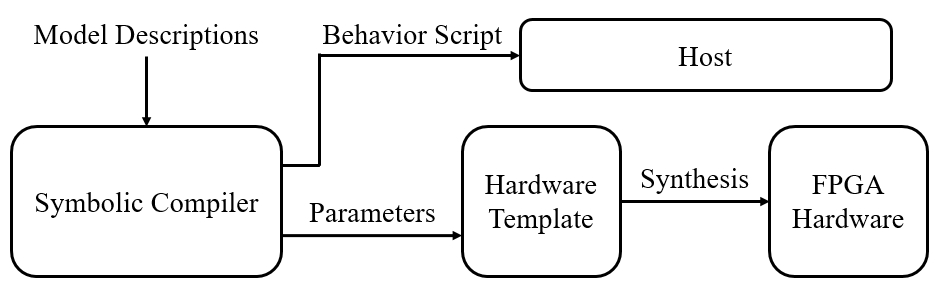
\includegraphics[width=1.0\linewidth]{./figure/framework.jpg}
	\caption{Overall fpDNN Framework}
	\label{framework}
\end{figure} 

$Model\ Mapper$ analyses U.S.E. to map the model onto hardware platform, and it generates the schedule and configuration for hardware kernels. 
Although storing model parameters and intermediate results in on-chip BRAM can significantly improve performance, we have to store them in on-board DRAM because 
we implement the whole model on a single FPGA board in this work and not enough BRAM is provided. Figure \ref{sc} shows an example of the working flow of \emph{Model Mapper}. Figure \ref{sc} (a) shows the U.S.E. for a fraction of VGG-19 \cite{vgg}, in which three convolution layers are executed. $Model\ Mapper$ takes the U.S.E., and generates the data flow graph with computation nodes (3 $Conv$) and data accessing nodes (4 $Data$) in Figure \ref{sc} (b). Due to the limitation on computation resource and DRAM storage, \emph{Model Mapper} must adopt resource reusing strategies. For computation resource reusing, $Model\ Mapper$ generates only one hardware kernel for each type of computation node, and maps all computation nodes of the same type to their corresponding kernels. The detailed kernel configurations are optimized and decided by performance model, which will be discussed in Section 4.1. For storage resource reusing, $Model\ Mapper$ divides DRAM into several data buffers, and reuses these buffers as long as no conflict occurs among these data accessing nodes. This mapping problem in essence equals to the well-known register allocation problem in compiler theory, which can be solved by DSATUR \cite{mapper} algorithm. The kernel schedule and kernel configuration are shown in Figure \ref{sc} (c).

\begin{figure}
	\centering
	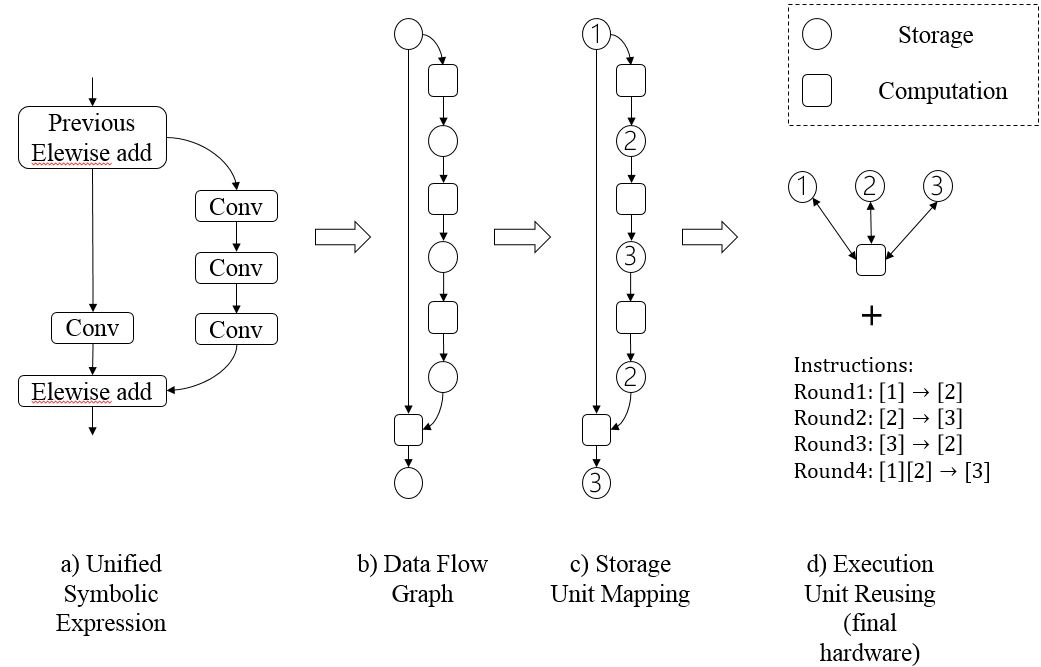
\includegraphics[width=1.0\linewidth]{./figure/sc.jpg}
	\caption{Working Flow of Model Mapper}
	\label{sc}
\end{figure}

$Software\ Generator$ takes kernel schedule to generate the C++ codes for $Host$, and the compiled C++ programs are in charge of execution scheduling for hardware kernels. Kernel configuration is used to instantiate hardware templates and generate corresponding OpenCL codes for $Device$. The whole fpDNN framework works in an ``end-to-end'' manner: from software-based model descriptions to FPGA-based model inference implementations. This procedure is all done automatically without any human intervention.

\section{Implementation}
The great complexity and variability of deep learning model structures have brought big challenges to generating optimal hardware for them individually. It is well-known that deep learning models are always constructed by stacked layers. These layers share similar structure at computation-intensive part, which can always be expressed as or converted into matrix multiplication. As a result, we divide the operations inside each layer into computation-intensive part and layer-specific part. For the computation-intensive part, we use a layer-independent matrix multiplication kernel ($MM$) to perform the calculations, like what cuDNN does. For layer-specific part, we implement data management kernels for each type of layer separately, which insures data are fed into $MM$ in a correct order. All these kernels work in a single-work item mode, which helps us to better control the behaviors and performance of kernels.

\subsection{MM Kernel}
The space complexity of storing matrices can be denoted as $O(N^2)$. However, while performing matrix multiplication normally without any optimization, input data are accessed repeatedly (i.e. I/O complexity $O(N^3)$), which makes I/O bandwidth become the performance bottleneck. To better explore the data locality, and make the limited DRAM bandwidth of modern FPGA board matches the computing power of $MM$, we take advantage of a tiling strategy to perform matrix multiplication. And the tiling strategy is also a promising solution for large-scale matrix multiplications, which can not be processed all at once with the limited on-chip resource.

Tiling strategy is generally shown in Figure \ref{tile}. The output matrix is tiled both in row and column, and the tiling size is denoted as $R_{tile}$ and $C_{tile}$ respectively. Then the two input matrices are tiled correspondingly to accomplish the matrix multiplication. To insure the computation are correctly performed in a tiling manner, we apply zero-padding to input matrices if any dimension of them is not divisible by its tiling size. In this tiling manner, input data can be easily buffered and reused on-chip, which simplifies the I/O complexity down to $O(N^2)$ and solves the I/O bottleneck.

\begin{figure}[h]
	\centering
	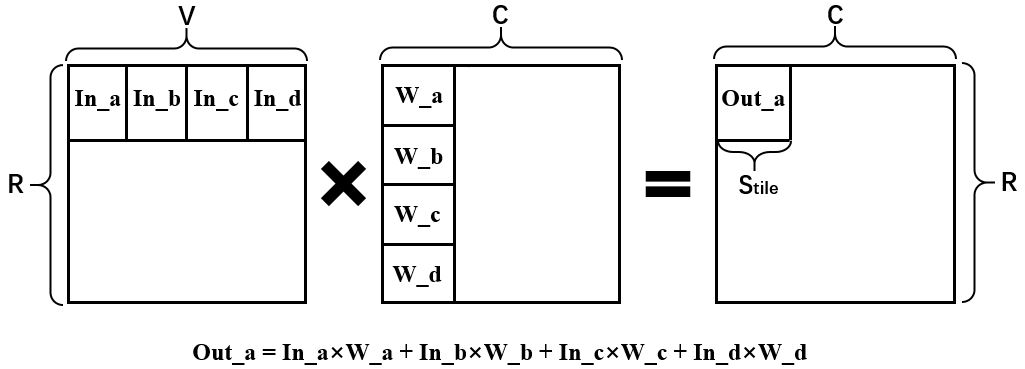
\includegraphics[width=1.0\linewidth]{figure/tile.jpg}
	\caption{Tiling Strategy for MM}
	\label{tile}
\end{figure}

Figure \ref{mm} shows the detailed structure inside $MM$. $MM$ takes in two tiles of input matrices, and performs the tiled matrix multiplication in $Dot\ Product\ Unit$ vector by vector. All the input data are fed into multipliers simultaneously, then the intermediate results are summed up through a reduction tree to minimize the computing latency. In practice, $N_{dot}$ $Dot\ Product\ Unit$s are generated, and they work simultaneously to increase the overall throughput. This degree of parallelism is decided by the trade-off between resource utilization and performance. Denoting the multiplication length of $Dot\ Product\ Unit$ as $L$, we can estimate the performance (in OPS, operations per second) of $MM$ in Equation \ref{perf}, where $Freq$ represents the running frequency of FPGA board.

\begin{figure}
	\centering
	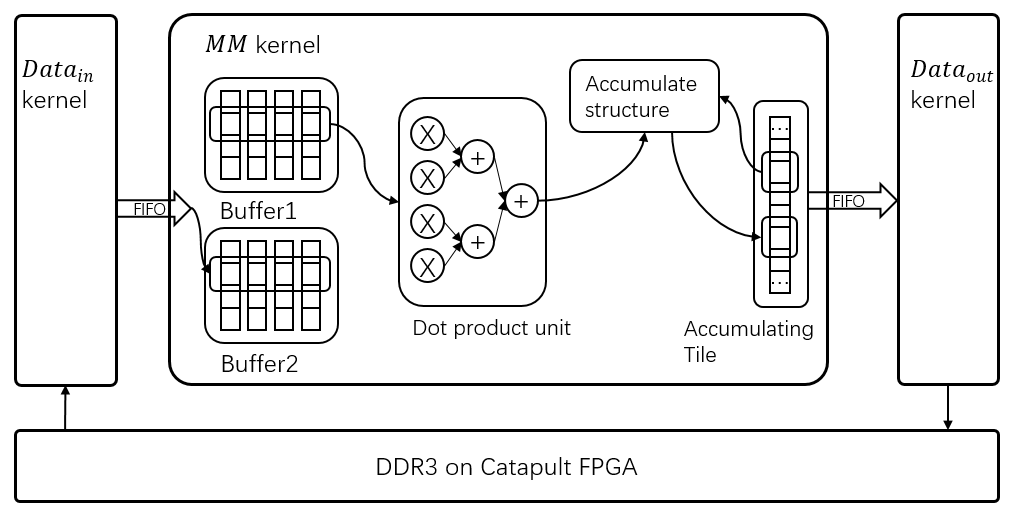
\includegraphics[width=1.0\linewidth]{./figure/mm.jpg}
	\caption{MM kernel}
	\label{mm}
\end{figure} 
\vspace{-15pt}
\begin{equation}
\centering
Performance\ =\ L \times N_{dot} \times 2  \times Freq
\label{perf} 
\end{equation}

\vspace{-10pt}Besides, we implement two on-chip buffers ($Buffer0$ and $Buffer1$ in Figure \ref{mm}) using two deep FIFOs. These two buffers are used to buffer the tiled input data, and they operate in a ping-pong manner: During a certain phase, $Dot\ Product\ Unit$ is processing with the tile fetched from $Buffer0$, and the tile to be processed in the next phase are loaded into $Buffer1$ simultaneously. Once \emph{Dot Product Unit} finished computing with current tile, it comes to the next phase, and every operation reverses. $Dot\ Product\ Unit$ processes the tile fetched from $Buffer1$, and $Buffer0$ loads the next tile. This ping-pong manner can overlap data communication with computation in time dimension, and significantly improves the throughput of $MM$. Thus, we can estimate the communication time ($T_{I/O}$) and computation time ($T_{Comp}$) for a tile by Equation \ref{Tio} and \ref{Tcomp} respectively, where $BW$ represents the data bandwidth between FPGA chip and DRAM.
\vspace{-5pt}
\begin{equation}
\centering
T_{I/O}\ =\ (R_{tile}+C_{tile})\times L/BW
\label{Tio} 
\end{equation}
\vspace{-10pt}
\begin{equation}
\centering
T_{Comp}\ =\ (R_{tile}\times C_{tile}\times L)/(L\times N_{dot})
\label{Tcomp} 
\end{equation}

\vspace{-10pt}The ping-pong manner requires that $T_{I/O}\ <\ T_{comp}$, and this equals to:
\vspace{-10pt}
\begin{equation}
\centering
BW\ >\ L\times N_{dot}\times(\dfrac{1}{R_{tile}}+\dfrac{1}{C_{tile}}) 
\end{equation}

\vspace{-10pt}Thus, several parameters ($R_{tile}$, $C_{tile}$, $L$, $N_{dot}$, and \emph{Freq}) can vary in different implementations. Each group of choices for these parameters corresponds to a possible configuration for hardware implementation, and these massive possibilities form a huge design space. \emph{Symbolic Compiler} in our fpDNN framework explores the whole design space for the optimal one. This exploration problem can be formulated as follows, and can be solved by heuristic algorithms for Pareto Optimality.
\vspace{-5pt}
\begin{equation}
\centering
\begin{split}
&Variables:\ R_{tile},\ C_{tile},\ L,\ N_{dot},\ Freq \\
&Constraints: \#\ of\ DSP,\ BW \\
&Target: \max(Performance)
\end{split}
\end{equation}

%This exploration work can be accomplished by simple algorithms for integer programming problems. \emph{Symbolic Compiler} in our framework can help to explore the design space and  find the optimal hardware configuration.

\subsection{Layer-Specific Data Management}
Deep learning models are constructed by many different types of layers, and the computation and data accessing pattern vary among these layers, so the strategies for converting them into $MM$ are also quite different. We provide details about the layer-specific data management strategies for typical types of layers as follows. 

\subsubsection{Convolution Layers}
The inference phase of convolution layers can be summarized as Equation \ref{conv} (bias adding is omitted for simplifying notations). These layers take a set of feature maps as input, and convolve these input with all the trained weights, then output a set of extracted feature maps.
\vspace{-8pt}
\begin{equation}
\centering
Out[x][y][z]=\sum_{i=1}^{N_i}\sum_{j=1}^{K}\sum_{k=1}^{K}In[i][y+j][z+k]*W[x][i][j][k]
\label{conv}
\end{equation}

\vspace{-10pt}To use the $MM$ kernel for the convolution layers, we need to convert the convolution operations into matrix multiplication, and the general strategy for converting a 2d-convolution into matrix multiplication is provided in Figure \ref{convert}. In this example, there are $N_{in}$ input feature maps and $N_{out}$ output feature maps. The size of convolution kernels is $K\times K$, and the sliding stride of convolution is $S$. Here is how we do the conversion: Firstly, we partition each output feature map into a single column of the output matrix. To calculate one pixel of one output feature map, we need a patch of input features (size of $K\times K\times M$) and a set of convolution kernels (size of $K\times K\times M$), so we partition a patch of input into a single row of input matrix and the corresponding set of convolution kernels into a single column of weight matrix. All these converting work and data address computing are done in data management kernels. Once the conversion is done,  we can use our $MM$ kernel to perform convolutions.

\begin{figure}
	\centering
	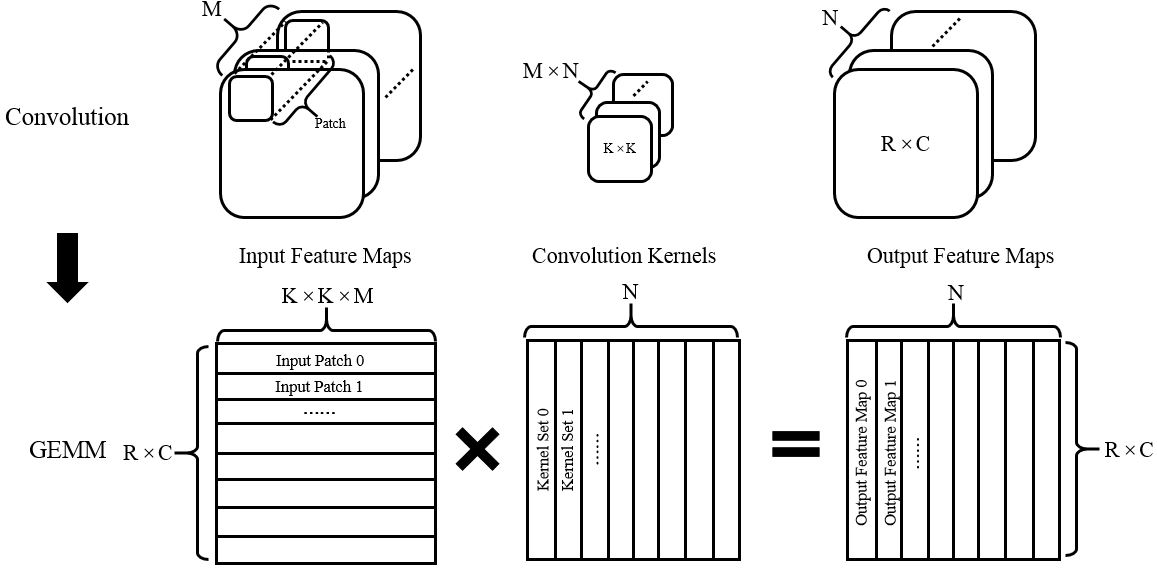
\includegraphics[width=1.0\linewidth]{./figure/convert.jpg}
	\caption{Converting Convolution into MM}
	\label{convert}
\end{figure}

Thus, we have to carefully manage the data accessing schemes to perform convolution with $MM$. However, these data management schemes usually need extra operations for address computation, and access DRAM in a random style, which brings great overhead on data fetching and storing. As a result, we propose to solve this tricky problem by optimizing data layout.

In Figure \ref{conventional} and \ref{datalayout}, we use a simplified example to illustrate the problem and our corresponding solution. We set $N_{in}=64$ and $K=2$ in our example. The size of input feature map is 3$\times$3, and the sliding stride of convolution kernel is 1. Conventionally, all input feature maps are stored in DRAM in a row-major manner, the detailed storage status is shown in Figure \ref{conventional}. We convert the convolution into matrix multiplication, and perform it in a tiled manner as described in Section 4.1. Here we set $R_{tile}=2$ and $L=8$. Prior work \cite{fpga'16} usually takes advantage of on-line address computing to fetch the proper data for $MM$. Thus, in each row within a tile, there are 8 input features, which can be viewed as a 2-dimension array, $L[2][K\times K]$ (dashed boxes in Figure \ref{conventional}). For the first layer, we illustrate the corresponding DRAM accessing pattern in Figure \ref{conventional}. Random accessing (like feature 5 to feature 9) occurs in every tile during the whole convolution. In practice, with a great number of feature maps and large-scale input features, this random accessing pattern occurs much more frequently. Random accessing can not fully utilize the efficiency of DRAM burst, and it also requires DRAM to recharge for long-stride address changing. Thus, this causes a sharp decrease on DRAM bandwidth. In our test, the actual bandwidth between DRAM and FPGA chip is restricted to about 1 GB/s, along with the extra address computation, this type of data layout makes I/O a more serious bottleneck of the overall performance.

\begin{figure}
	\centering
	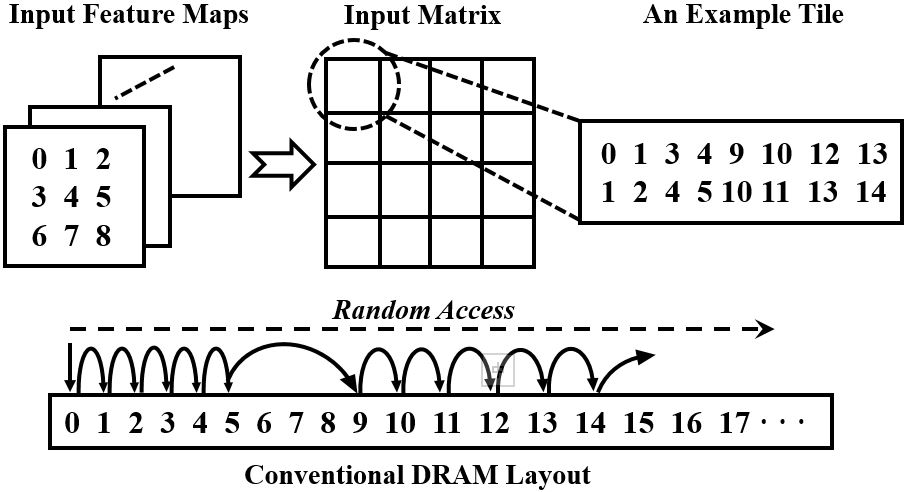
\includegraphics[width=1.0\linewidth]{./figure/conventional.jpg}
	\caption{Conventional Layout and Accessing Pattern}
	\label{conventional}
\end{figure}

\begin{figure}
	\centering
	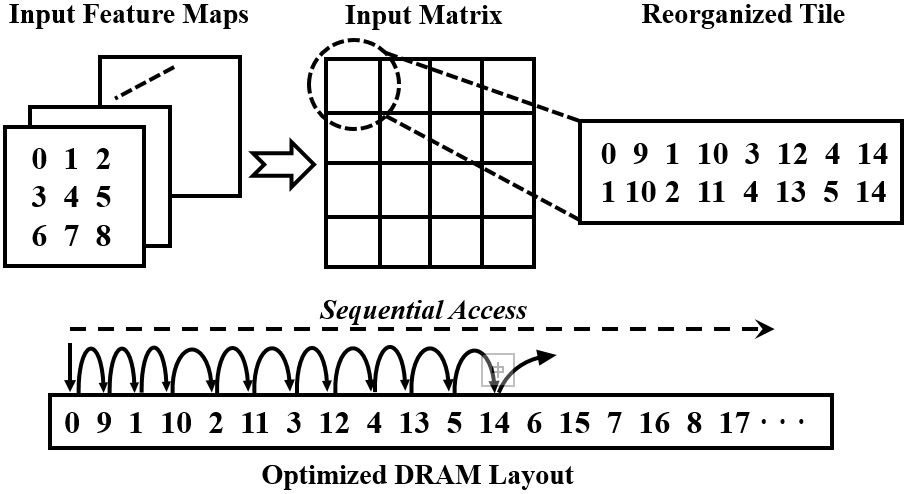
\includegraphics[width=1.0\linewidth]{./figure/layout.jpg}
	\caption{Optimized Layout and Accessing Pattern}
	\label{datalayout}
\end{figure}

To issue this problem, we optimize the data layout of input feature maps. The result after data layout optimization is generally shown in Figure \ref{datalayout}. For each row within a tile, we reorganize the 2-dimension input array from $L[2][K\times K]$ to $L[K\times K][2]$ (dashed boxes in Figure \ref{datalayout}). In other words, we packed the features at the same position of each feature map together, and store them in DRAM group by group to fit the characteristics of sliding convolution kernel. The corresponding DRAM storing status is also shown in Figure \ref{datalayout}. Thus, with the optimized data layout, the data accessing pattern is in a sequential way. The other input matrix of convolution, weight matrix, need to be adjusted accordingly, but the overhead brought by this can be ignored since weights are pre-trained and these adjustments can be applied before model deployment. Furthermore, with this data layout optimization, most features overlaps in consecutive tiles, and we just need to buffer the previous tile and fetch an extra feature to cook up the next tile. This can further save DRAM access by nearly $(K-1)/K$.

%The effective bandwidth with and without this data layout optimization is compared in Table \ref{ebw}.
We test this optimization for data layout, and the actual bandwidth between DRAM and FPGA chip is improved to about 8 GB/s.
It is obvious that this data layout optimization optimizes the bandwidth constraint greatly, and the bottleneck of the whole system turns to the computation part.

\subsubsection{LSTM Layers}
In recent years, Long Short-Term Memory (LSTM) has gained great popularity in RNN design. These LSTM-RNNs use LSTM cells in their topological structure, and achieve state-of-the-art performance in several applications. Numerous variants of LSTM structures have been proposed, while \cite{lstmsum} finds that all these variants show little difference in model accuracy. So we implement the LSTM cell described by Equation \ref{lstmgate} to \ref{lstmout} (bias adding is omitted for simplifying notations), which is also the implementation in \cite{lstm}. The input of LSTM layer is the combination of input vector at current time-step ($In_t$) and cell vector at previous time-step ($C_{t-1}$). Then LSTM layer multiplies input with different weight matrices to get the output vectors of four gates: input gate ($I_t$), forget gate ($F_t$), output gate ($O_t$), and cell gate ($\tilde{C_t}$). Then these output vectors generate the final output vector of LSTM layer through element-wise operations described in Equation \ref{lstmout}.
\vspace{-5pt}
\begin{equation}
\centering
\begin{pmatrix}
I_t\\
F_t\\
O_t\\
\tilde{C_t}\\
\end{pmatrix}
=
\begin{pmatrix}
sigmoid\\
sigmoid\\
sigmoid\\
tanh   \\
\end{pmatrix}
\begin{pmatrix}
Weight_I\\
Weight_F\\
Weight_O\\
Weight_C\\
\end{pmatrix}
\times
\begin{pmatrix}
In_t\\
C_{t-1}\\
\end{pmatrix}
\label{lstmgate}
\end{equation}
\vspace{-10pt}
\begin{equation}
\centering
Out[x]\ =\ O_t[x]\times tanh(F_t[x]\times C_{t-1}[x]+I_t[x]\times \tilde{C_t}[x])
\label{lstmout}
\end{equation}

\vspace{-10pt}As a result, the main computation inside LSTM layers is matrix multiplying vector. Unfortunately, this operation is inefficient
in terms of data locality, because every weight element fetched from DRAM is used only once. We solve this problem by batching input vectors during inference as below, and every element of weight matrices is reused $N_{batch}$ times.
\vspace{-6pt}
\begin{equation}
\centering
Weight \times In \rightarrow Weight \times (In^1, In^2, \dots, In^{N_{batch}})
\end{equation}

\vspace{-10pt}In this batching manner, we can easily convert matrix multiplying vector into matrix multiplication, and reuse $MM$ kernel to perform it. Besides, to further explore the specific data flow property of LSTM, we apply two special strategies to the kernel for writing data back to DRAM.

Firstly, Equation \ref{lstmout} indicates that there is no need to buffer the gate vectors ($I_t$, $F_t$, $O_t$, and $\tilde{C_t}$), since each element inside gate vectors is used exactly once in element wise operations to generate $Out$. In practice, we arrange these vectors as below so that $MM$ outputs them together and data management kernels process them to get the $Out$ immediately.
\vspace{-10pt}
\begin{equation}
\centering
\begin{pmatrix}
I\\
F\\
O\\
\tilde{C}\\
\end{pmatrix}
\xrightarrow{In\ MM}
\begin{pmatrix}
I^0_0\ I^1_0\ \cdots\ I^M_0\\
F^0_0\ F^1_0\ \cdots\ F^M_0\\
O^0_0\ O^1_0\ \cdots\ O^M_0\\
\tilde{C}^0_0\ \tilde{C}^1_0\ \cdots\ \tilde{C}^M_0\\
\vdots\ \vdots\ \ddots\ \vdots\\
I^0_N\ I^1_N\ \cdots\ I^M_N\\
F^0_N\ F^1_N\ \cdots\ F^M_N\\
O^0_N\ O^1_N\ \cdots\ O^M_N\\
\tilde{C}^0_N\ \tilde{C}^1_N\ \cdots\ \tilde{C}^M_N\\
\end{pmatrix}
\label{lstmlayout}
\end{equation}

\vspace{-10pt}Secondly, LSTM adopts $tanh()$ and $sigmoid()$ as activation functions, which are quite resource-expensive for hardware implementation. However, we notice that activation occupies only a small portion of the whole calculations during model inference. Thus, we instantiate a small amount of activation computing units at data output kernel, which are just enough to keep up with the throughput of $MM$. Taking advantage of this approach, we use full-precision version of $sigmoid()$ and $tanh()$ instead of linear approximation in previous work \cite{fccm'15}. We insert a deep FIFO (size of an output tile) between $MM$ and data output kernel, and this FIFO decomposes the computing process inside two kernels, making both kernels always work at full load asynchronously.


\subsubsection{Fully-Connected Layers}
The inference phase of fully-connected layers can be summarized as Equation \ref{fc}, (bias adding is omitted for simplifying notations). These layers output a vector ($Out$) as the product of input vector ($In$) and weight matrix ($Weight$). Fully-connected layers are also widely deployed in deep learning models. Layers inside ANNs, classifiers inside modern CNNs, and recurrent layers inside simple RNNs are all in fact fully-connected layers. As a result, we apply the same implementation strategies to these layers. As shown in Equation \ref{fc}, computation inside fully-connected layers can be viewed as matrix multiplying vector. Thus, we can use our $MM$ kernel to perform it by similar strategies of LSTM layers. 
\vspace{-5pt}
\begin{equation}
\centering
Out[x]=\sum_{i=1}^{N_i}In[i]\ *\ Weight[x][i]
\label{fc}
\end{equation}

\subsubsection{Pooling Layers}
The operations performed in pooling layers can be summarized as Equation \ref{pool}. Typically, pooling layers take the maximum (max-pooling) or the average (average-pooling) of the input features in a pooling window as output. Pooling layers are always responsible for sub-sampling features. As shown in Equation \ref{pool}, though not much computation is involved in pooling layers, pooling window usually strides on a 2D address space. As a result, it is quite complex and inefficient to add pooling operations to data output kernel directly, and we implement an individual pooling kernel instead for flexibility and extensibility.
\vspace{-3pt}
\begin{equation}
\centering
Out[x][y]= \mathop{Pooling_{Max/Average}}\limits_{0\leqslant i,j<Size_{window}}(In[x+i][y+j])
\label{pool}
\end{equation}

\subsubsection{Activation Layers}

The operations in activation layers are always element-wise functions applied to the features: $tanh()$, $sigmoid()$, $ReLU()$, etc. Thus, there is no need to implement an extra kernel for them or convert them into $MM$. We simply add them to data output kernel before the outputs are written back to DRAM. It is worth noting that the total number of operations inside activation layers is much smaller than that inside $MM$, so we allocate a small portion of computation resource to activation layers as what we do for activation functions in LSTM layers.

%The operations in activation layers are always element-wise functions to the features, so there is no need to implement an extra kernel for it or convert it into MM. We simply add them to $Data_{out}$ before the outputs are written backc. However, there are several types of activation functions. For simpler ones like ReLU ($tensorflow.nn.relu()$ in TensorFlow), we implement them directly as they are. For ones including complex exponential operations like tanh ($tensorflow.tanh()$ in TensorFlow) and sigmoid ($tensorflow.sigmoid()$ in TensorFlow), we use linear approximation [cite] to further improve performance and resource utilization, which is also a common optimization for hardware implementation \cite{fccm'15}. The experiments show that the accuracy loss is XX\%, which is small enough to be ignored.
\begin{table*}[!htb]
	%	\scriptsize
	\centering
	\begin{tabular}{|c|c|c|c|c|c|c|}
		\hline
		& \cite{fpga'15} & \cite{fpga'16} & \cite{aeye} &  \multicolumn{3}{|c|}{Our Imp.}\\
		\hline
		FPGA chip & Virtex-7 VX485T& Stratix-V GSD8 & Zynq XC7Z045 & \multicolumn{3}{|c|}{Stratix-V GSMD5}\\
		\hline
		Frequency & 100MHz & 120MHz & 150MHz & \multicolumn{3}{|c|}{200MHz}\\
		\hline
		CNN size & 1.33GOP & 30.90GOP & 30.76GOP & \multicolumn{3}{|c|}{39.20GOP}\\
		\hline
		Precision & float32 & fixed8-16 & fixed16 &  float32 & fixed16 & fixed8\\		
		\hline
		Performance & 62GOP/S(Convolution Only) & 118GOP/S & 137GOP/S & 81GOP/S & 173GOP/S & 315GOP/S \\
		\hline
	\end{tabular}
	\caption{CNN Performance Comparison with Prior Work}
	\label{cnn}
\end{table*}

\section{Evaluation}
To illustrate the effectiveness and great performance achieved by our proposed fpDNN framework, we design and implement several models as our case studies for modern typical deep learning structures. 

\subsection{Experimental setup}
For the software part, the $Symbolic\ Compiler$ that performs performance estimation, parameter decision, and OpenCL code generation is written in Python. To implement our design on FPGA board, we take advantage of a high-level synthesis design tool, Altera AOCL. This high-level synthesis tool helps us synthesis and implement the OpenCL-based codes into FPGA programming files. The codes on the host is written in C++, and compiled by Visual Studio 2013.

For the hardware part, we use an Altera Stratix-V GSMD5 FPGA with a 4GB DDR3 DRAM as external storage. The FPGA logic clock frequency is set to 200MHz, and the run-time power of the FPGA board is about 25W. This FPGA board is plugged into a PCI-e Gen2 x8 slot of a host computer. 

For performance comparison, we use TensorFlow(r0.8) to run model inference on both CPU and GPU. We use a server that includes 2 processors for the CPU implementation, and each processor is a 6-core Xeon E5-2620@2.4GHz with a 15MB L3 cache. The run-time power of each processor is about 95W. The GPU card is an NVIDIA GeForce GTX TITAN X, which has 3072 cores and 12GB GDDR5 memory. The run-time power of it is about 250W. Both CPU- and GPU- implementations run with batch size set to 256.


\subsection{Experimental results}

\subsubsection{Performance}
$MM$ kernel is the core part of our FPGA-based model inference, so we compared the performance of our $MM$ kernel with other state-of-the-art implementations. We show the performance (in GOP/S) of our implementations, Intel MKL \cite{mkl} and Altera example design for matrix multiplication \cite{altera} in Figure \ref{performance}. Our implementation and Altera example design run on the same FPGA board, and Intel MKL runs on the CPU introduced in Section 5.1. As shown in Figure \ref{performance}, when matrix size raises to a large scale,our 32-bit, 16-bit, and 8-bit implementations of $MM$ can outperform Altera example design by 3.14x, 6.28x and 12.55x respectively. The 8-bit implementation outperforms Intel MKL by 1.81x on average, and the performance of 16-bit implementation is close to that of Intel MKL. The resource utilization of our $MM$ implementations are shown in Table \ref{resource}.

\begin{figure}
	\centering
	\includegraphics[width=1.0\linewidth]{./figure/performance.jpg}
	\caption{MM Performance Comparison}
	\label{performance}
\end{figure}

\begin{table}
	\centering
	\begin{tabular}{|c|c|c|c|}
		\hline
		Precision & float32 & fixed16 & fixed8\\
		\hline
		Logic & 164100(95\%) & 85762(50\%) & 82595(48\%)\\
		\hline
		BRAM & 1343(67\%) & 919(46\%) & 859(43\%)\\
		\hline
		DSP & 264(17\%) & 1036(65\%) & 524(33\%)\\
		\hline
	\end{tabular}
	\caption{Resource Utilization of MM}
	\label{resource}
\end{table}

To show the performance of our fpDNN framework on a complete model, we firstly compare our CNN implementations with previous accelerators, as shown in Table \ref{cnn}. We implement VGG-19 \cite{vgg}, which has 16 convolution layers, 3 fully connected layers and 5 max pooling layers. From Table \ref{cnn}, we can conclude that the implementations generated by our fpDNN framework achieve state-of-the-art performance even when compared with hand-coded accelerators.

Note that numerous prior works \cite{eie} \cite{handeep} have shown that the accuracy of deep learning models is robust enough with a decrease in data precision. Many previous works on accelerating deep learning model inference \cite{fpga'16} \cite{aeye} used fixed-point parameters in their design for performance improving and resource saving. Recent research finds that deep CNN models can even use binary values for model inference without much accuracy loss \cite{bnn} \cite{xnor}. So in our implementation, we also support implementing fixed-point versions of the target model. Designers using our fpDNN framework can specify the fixed-point precision by simply using the ``$-fixed\_point$'' compilation option in our \emph{Symbolic Compiler}. However, the accuracy loss brought by data quantization must be estimated and tested by the users in advance, and we leave it to the users to make a decision on the trade-off between accuracy and performance.

\subsubsection{Platform Comparison}
To show the great performance and energy efficiency provided by our fpDNN framework, we compare our implementations with those on CPU and GPU in Table \ref{ee}. We implement several deep learning models as benchmarks: VGG-19 \cite{vgg} (CNN), LSTM \cite{lstm} (RNN), Res-152 \cite{drn} (Residual Net). The energy efficiency is measured in GOP/J (giga ops per joule). Table \ref{ee} shows that: for single-precision (float32) implementations generated by our fpDNN framework, the energy efficiency is higher than CPU in all models, while higher than GPU only in Res-152, and this may be caused by the cross-layer residual short-cuts in Res-152. For low-precision (fixed16 and fixed8) implementations, our fpDNN framework can easily beat TensorFlow implementation CPU and GPU in energy efficiency.

\begin{table}
	%	\scriptsize
	\centering
	\begin{tabular}{|c|c|c|c|c|c|}
		\hline
		Model & \multicolumn{5}{|c|}{VGG-19\cite{vgg}}\\
		\hline
		Platform & CPU & GPU & \multicolumn{3}{|c|}{FPGA}\\
		\hline
		Pecision & float32 & float32 & float32 & fixed16 & fixed8 \\
		\hline
		GOP/S & 119 & 1704 & 81 & 173 & 315\\
		\hline
		GOP/J & 0.63 & 6.82 & 3.24 & 6.92 & 12.6\\
		\hline
		Model & \multicolumn{5}{|c|}{LSTM\cite{lstm}}\\
		\hline
		Platform & CPU & GPU & \multicolumn{3}{|c|}{FPGA}\\
		\hline
		Pecision & float32 & float32 & float32 & fixed16 & fixed8 \\
		\hline
		GOP/S & 103 & 1828 & 86 & 188 & 396\\
		\hline
		GOP/J & 0.54 & 7.31 & 3.44 & 7.52 & 15.84\\
		\hline
		Model & \multicolumn{5}{|c|}{Res-152\cite{drn}}\\
		\hline
		Platform & CPU & GPU & \multicolumn{3}{|c|}{FPGA}\\
		\hline
		Pecision & float32 & float32 & float32 & fixed16 & fixed8 \\
		\hline
		GOP/S & 119 & 1661 & 73 & 135 & 237\\
		\hline
		GOP/J & 0.63 & 6.60 & 2.92 & 5.40 & 9.48\\
		\hline
	\end{tabular}
	\caption{Performance Comparison on Different Platforms}
	\label{ee}
\end{table}

\subsubsection{Framework Effectiveness}
For all the implemented models in Table \ref{ee}, fpDNN takes about 4-5 hours to generate the FPGA programming files as well as the host programs from the TensorFlow-described models. When only model configuration changes, it costs fpDNN only several minutes to regenerate a new kernel schedule instead of regenerating a new hardware. It may take an experienced hardware engineer several weeks to implement a new deep learning model on FPGAs before a comprehensive design space exploration. So our fpDNN framework can improve the efficiency of deep learning models' deployment significantly.
Besides, our fpDNN framework can support all the typical types of deep learning models and much deeper models like Res-152, so fpDNN can provide much greater flexibility, scalability and productiveness compared with hand-coded implementations. To the best of our knowledge, it is the first FPGA implementation of Res-152 in literature.
Furthermore, deep learning researchers or software developers with little knowledge about FPGA implementation can easily use this fpDNN framework to get a highly efficient implementation of their pre-trained models. Thus, our fpDNN framework can be widely popularized.

%The accuracy of the estimation models in \emph{Symbolic Compiler} is evaluated in Figure \ref{estimate}. We show the comparison between estimated performance and measured performance of implemented models in Section 5.2.2, and we can see that our proposed models are accurate enough with only XX \% error.

%\section{Related work}
\vspace{-3pt}
\section{Conclusions and future work}
In this paper, we propose a framework that automatically compiles deep learning models onto FPGAs to accelerate model inference. We also propose a high-performance matrix multiplication kernel and carefully-designed data management strategies. Several accurate performance models are developed for choosing the optimal hardware configuration. Our case studies show the great performance and effectiveness achieved by this framework.

For future research, we will firstly go on working with a distributed version of this framework on an FPGA fabric. Secondly, we will adapt the kernels inside our fpDNN framework to support emerging optimization techniques for deep learning models like pruning, binarization, etc. Thirdly, we will further extend our fpDNN framework to model training.


%ACKNOWLEDGMENTS are optional
%\section{Acknowledgments}

%
% The following two commands are all you need in the
% initial runs of your .tex file to
% produce the bibliography for the citations in your paper.
\scriptsize
\bibliographystyle{abbrv}
\bibliography{sigproc}  % sigproc.bib is the name of the Bibliography in this case
% You must have a proper ".bib" file
%  and remember to run:
% latex bibtex latex latex
% to resolve all references
%
% ACM needs 'a single self-contained file'!
%

% That's all folks!
\end{document}
